\textbf{شبکه عصبی (18نمره)}



در این سوال می‌خواهیم یک شبکه عصبی طراحی کنیم تا با دریافت ۴ مقدار، مرتب‌ شده‌ی آن‌ها را خروجی بدهد.

آ) ابتدا با مسئله مرتب‌سازی دو عدد شروع می‌کنیم. شبکه‌ی عصبی زیر زوج مرتب $(x_1, x_2)$ را به عنوان ورودی می‌گیرد و زوج مرتب $(y_1, y_2)$ را به عنوان خروجی بر می‌گرداند به گونه‌ای که $y_1 = \max(x_1, x_2)$ و $y_2 = \min(x_1, x_2)$ می‌باشند. وزن‌ها و اریبی‌ها\footnote{bias} و توابع فعال‌سازی را در این شبکه مشخص کنید. (لازم نیست که توابع فعال‌سازی در هر لایه یکسان باشند)
\begin{align*} 
    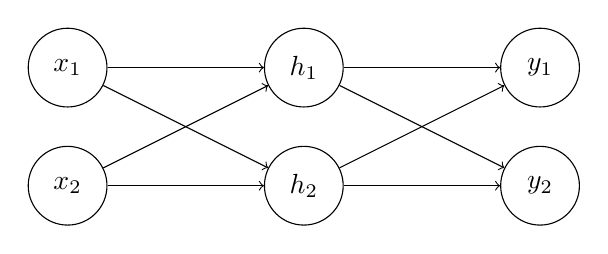
\begin{tikzpicture}[scale=1, transform shape] 
        % Input Layer 
        \foreach \m/\l [count=\y] in {1,2} \node [circle, draw=black, fill=white!30, minimum size=10mm] (input-\m) at (0,-\y*1.5) {$x_\m$}; 
        % Hidden Layer 
        \foreach \m [count=\y] in {1,2} \node [circle, draw=black, fill=white!30, minimum size=10mm] (hidden-\m) at (3,-\y*1.5) {$h_\m$}; 
        % Output Layer 
        \foreach \m [count=\y] in {1,2} \node [circle, draw=black, fill=white!30, minimum size=10mm] (output-\m) at (6,-\y*1.5) {$y_\m$}; 
        % Connect input to hidden layer 
        \foreach \i in {1,2} \foreach \j in {1,2} \draw[->] (input-\i) -- (hidden-\j); 
        % Connect hidden to output layer 
        \foreach \i in {1,2} \foreach \j in {1,2} \draw[->] (hidden-\i) -- (output-\j); 
    \end{tikzpicture} 
\end{align*}


ب) اکنون با استفاده از شبکه ساخته شده در بخش آ، شبکه عصبی $f$ را طراحی می‌کنیم تا با دریافت ورودی $(x_1, x_2, x_3, x_4)$ مقادیر مرتب شده $(y_1,y_2,y_3,y_4)$ را به عنوان خروجی بازگرداند. گراف این شبکه را رسم کنید. (برای انجام این کار می‌توانید شبکه پیاده‌سازی شده در بخش پیش را به عنوان یک ماژول در نظر بگیرید)